\documentclass[12pt]{article}
\usepackage{graphicx} % Required for inserting images
\usepackage[margin=1in]{geometry}
\usepackage{xcolor}
\usepackage{listings}
\usepackage{minted}
\usepackage{xparse}
\usepackage{graphicx}
\usepackage[normalem]{ulem}
\usepackage{soul}
\usepackage{float}
\usepackage{hyperref}
\NewDocumentCommand{\codeword}{v}{%
\texttt{\textcolor{blue}{#1}}%
}
\usepackage{hyperref}

\title{CMSC838L - Final report}
\author{Arjun Vedantham \\ Yusuf Bham}
\date{May 2024}

\begin{document}

\maketitle

\section{Introduction and Motivation}
Digital signal processing techniques are extremely important in telecommunications, computer vision, and a number of other related fields.
In particular, digital signal processing techniques form a key component behind the idea of software defined radio (SDR),
which refers to analyzing digital samples that represent radio signals with software, instead of discrete hardware components that operate
over signals in analog formats. Software defined radio presents a notable improvement in flexibility for radio engineers, and removes the
need for specialized hardware components - instead, new signal demodulation techniques or formats can be deployed just through a simple software
update.

SDR users typically define signal processing pipelines using platforms like GNURadio. GNURadio presents a graphical format for creating these
pipelines, with discrete blocks representing a signal source, signal sink, or an intermediate step in the processing pipeline. As an example,
see the "flowgraph" (as called in GNURadio's documentation) below. This starts by instantiating a signal source from an RTL-SDR (a type of hobbyist SDR that can be used
over USB with consumer PCs), and sets both a sampling rate (32000 Hz) and a listening frequency (signals at 433 MHz). From here, these samples
are fed into a low pass filter block (which smooths out high frequency noise in the signal), and the resulting signal is transformed into
a stream that is passed to a GUI block that graphs the signal, using a Fast Fourier Transform (FFT) to move the signal into the frequency domain.

This simple flowgraph is stored in an XML format, and is used by GNURadio's backend to generate a Python script that actually runs the defined
processing pipeline. In addition, there are also C/C++ modules loaded into the runtime system for low level tasks - for instance, a USB driver for the SDR.

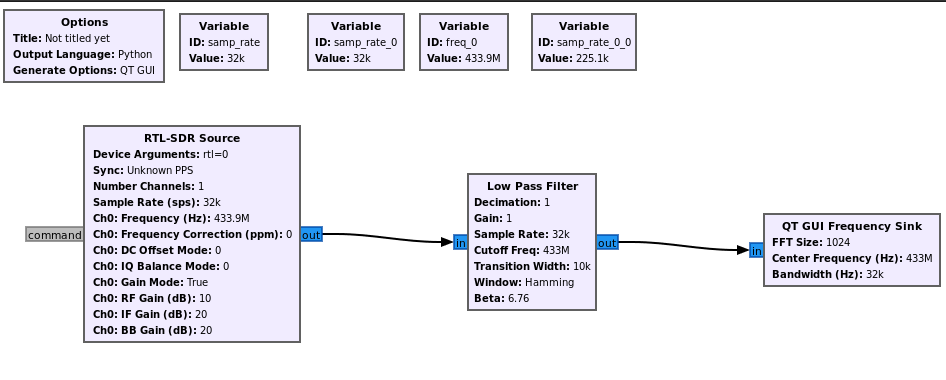
\includegraphics[width=\linewidth]{images/gnuradio.png}

\subsection{Problems Identified with State of the Art}
There are number of problems with this current approach. First, GNURadio's practice of emitting Python scripts means that parallelism is
limited on two fronts - first, because of language design choices (Python's infamous "global interpreter lock", which essentially forbids
runtime concurrency), and also because we are ultimately running this script on standard PC hardware, which uses an inherently sequential
von Neumann architecture. Additionally, as previously mentioned, there is also an extensive library of C/C++ modules, and the implementation
of these modules are opaque to the Python-level code generated by GNURadio's flowgraph compiler.

As such, we identified two research questions that we aimed to answer in this project:

\begin{itemize}
    \item Could we use hardware acceleration to get better performance and greater parallelism for DSP applications?
    \item Could we design a language that is more conducive to defining correct DSP pipelines?
\end{itemize}

\section{Literature Review}
We started by conducting a literature review of existing languages designed for DSP problems.
\subsection{Ziria}
One of the first papers we considered as Ziria, a domain specific language that was
designed to aid development in implementations of the physical layer of wireless protocols.
Ziria presented a functional language design syntax, and was specifically intended for wireless protocol
implementations on IOT hardware. As such, it contained many primitives that we thought would
be important to add to our language - for instance, an "FFT" primitive function. However Ziria had a key limitation -
it was designed for standard CPUs, which meant that there were still parallelism limitations.

\subsection{Calyx}
One technique generally used for hardware acceleration for specialized applications like this
is to deploy them to FPGAs. One example of this was the Catapult paper that we read in class,
where Microsoft deployed FPGAs to accelerate running PageRank as part of their Bing server infrastructure.
However, FPGAs are notoriously difficult to program, and generally require extremely fine-grained circuit
configurations written in a hardware description language like Verilog.

Calyx is an intermediate representation for compilers developed by the CAPRA research group at Cornell.
It defines circuits in three distinct parts - a collection of memories (consisting of combinational memories/
flip-flops and registers), wire groups (which denote assignments between different memory components
in the circuit), and a statically defined control schedule that orders wire assignments.
Calyx has already been used in the Filament HDL, another domain specific language project from the CAPRA
group that incorporated signal timing into the language's type system.

\section{Technical Contribution}
We decided to use the Calyx IR and design a more general, hardware acceleratable language for DSP tasks, called Zinnia.
\footnote{Named "Zinnia" because "calyx" refers to the petals of a flower and zinnias are a type of flower. Plus it sounds like Ziria.}
We also considered emitting circuits using CIRCT, the LLVM framework that allows compilers to generate
MLIR that is subsequently lowered to a Verilog hardware description, however we quickly found that
CIRCT lacked the project maturity needed to develop even a basic language around it. This included
no binaries to link against, thus requiring us to compile a large subset of the LLVM project, which was not practical.
Calyx also had better documentation for its IR, and a small standard library of memory cells that could be easily integrated
into circuits synthesized when the compiler lowers from the IR to a Verilog hardware description.
\subsection{Code Generation}
The compiler that we wrote for Zinnia traverses the AST recursively. Since there is no concept of dynamic
memory allocation for circuits, we focused on generating the required memories for the circuit first.

Additionally, while Calyx has a "par" primitive for parallelizing parts of the circuit, Zinnia currently only generates
circuits using the "seq" ("sequential") control flow keyword for easier debugging and testing. Even though parallelism
at the user level is limited, we still hoped to expose some of the potential parallel speedups through the use
of a function primitive that could be used to get implicit parallelism.

\subsection{Prefix Sums Scan}
To expose some parallelism without explicitly supporting copmiling using the "par" control flow block,
we implemented a version of parallel scan using the prefix sums algorithm.

\section{Evaluation}
We decided to evaluate our language in three different ways: correctness testing, scalability testing, and hardware testing.
\subsection{Correctness Testing}
To verify the correctness of the language, we used the Cocotb RTL testing framework. This allows
us to run a simulated version of the circuit's clock and write unit tests around elements of the circuits
that we generate.
\subsection{Scalability Testing}
Second, we focused on testing scalability. For this, we focused on evaluating the "scan" primitive, since
it is the main way end-users would be able to obtain parallelism through the language (at least, as it is currently implemented).
We found that in simulation, our parallel scan implementation always took 71 cycles to generate outputs, given a set of 8 integers
to iterate over. While parallel scan theoretically provides work bounds of $O(n)$ and span bounds of $O(lg(n))$, in practice the
work and span bounds of our implementation are worse. This is because we were not sure if it was possible to instantiate
an arbitrarily high number of registers, so we focused on using the combinational memory primitives to hold intermediate values
(particularly between the "sweep-up" and "sweep-down" phases of parallel scan). Combinational memory primitives in the Calyx IR
are exclusive read/write memory cells, and take at least one cycle to set the data address and read the stored value out of the memory
into a register. This restriction essentially limited the parallelism that we could achieve to only a few steps of the algorithm - specifically,
summing values between nodes at each level of the prefix sums tree, since the additions were purely combinational and depended only
on values in registers that were ready to go at the last cycle.
\subsection{Physical Testing}
We hoped to eventually deploy circuits that were synthesized using Zinnia to a Lattice Icestick FPGA.
This FPGA can be used with consumer devices over a USB connection, and has a large library of open source tooling.
This includes the Yosys synthesis toolkit (which handles transforming high level Verilog hardware descriptions into
lower level RTL circuits), the nextpnr place and route tool (which handles connections between logic units
on the FPGA), and iceprog, an open source programming tool that could deploy circuits with complete routing
to the flash memory on-board the Icestick.

Circuits synthesized by Calyx include three signals by default - a "go" line, which when activated,
activates the circuit, a "clk" (clock) line, which handles cycle-level signalling for the sequential logic
elements of the circuit, and a "reset" line, which can be used to reset the circuit while active.

In order to actually use the synthesized circuits, the "go" line must be pulled to logical high, and
while the reset lines needed to be set to logical low, and the clock line must be tied to the 12 MHz
oscillator built into the Icestick. Values for the "scan" primitive could then be loaded in from the Icestick's
block RAM module.

To support dynamically loading values into block RAM, we wrote a small serial communication driver for the Icestick.
Specifically, this was a form of one way (half-duplex) SPI, with an Arduino serving as the primary device on the SPI
bus, and the Icestick serving as the secondary device. We chose SPI because it is relatively easy to implement
on the receiving side (in fact, a shift register is enough to receive data transmitted over the data line).
While testing the SPI driver, we wanted to use an external clock source to control the speed of data transmission,
and ensure that the Icestick was sampling the data line in phase with the transmitting device's clock (in this case
an Arduino). Unfortunately, setting the clock line for the circuit loaded onto the FPGA also sets the clock line
for the USB programmer chip, which requires a 12MHz signal in order to function correctly. This misconfiguration
prevented us from loading new circuits onto the FPGA, and required us to use simulation as our primary evaluation
method instead.

\section{Conclusion}
In the end, we were able to implement a version of the scan primitive in the Calyx IR, implement a bidirectional
typing system, add some basic language features into our language, and use external circuit verification and simulation
tools to show that our circuits performed as the high level program specified.

However, there is still room for improvement - we do not have support for looping structures, even though the Calyx IR supports
it. We were also not able to show our circuits running on real hardware, which was the ultimate goal of the project.

One obstacle that we did not foresee was the difficulty of working with the Calyx IR from Rust. While LLVM's CIRCT project
has a robust Rust API, it seems that the authors of the Calyx IR primarily want language authors to use their IR from
a Python builder module or the CIRCT toolchain, even though the Filament HDL (which was authored by the same research
group and uses Calyx as its IR) is also written in Rust. For some issues, like linking against the combinational memory
primitives or inlining other components, the Rust library documentation was so poor that we ended up looking through
Filament's implementation and using that as a guide for building our compiler.
\end{document}
